%\documentclass[A4,12pt]{article}
\documentclass[letterpaper,12pt]{article}
\usepackage{epsfig}
\usepackage{float}
\usepackage{amssymb,amsmath,latexsym}
\usepackage[labelformat=empty]{caption}
\usepackage{color}
\usepackage{CJKutf8}
%\usepackage[abs]{overpic}

\usepackage{graphicx}
\usepackage{epstopdf}

\usepackage{tikz}
\usetikzlibrary{arrows}
\usetikzlibrary{calc}
\usetikzlibrary{scopes}
\usetikzlibrary{shadows}
\usetikzlibrary{chains}
%\usetikzlibrary{shadows.blur}

\topmargin      0in 
\textheight     9.0in 
\headheight     -0.0in 
\headsep        0in
\textwidth      6.5in 
\oddsidemargin  0in 
\evensidemargin 0in
\parskip        0pt

\newcommand{\slfrac}[2]{\left.#1\middle/#2\right.}
\newcommand{\bm}    [1]{\mbox{\boldmath $#1$}}

\newtheorem{thm}           {Theorem}
\newtheorem{lemma}    [thm]{Lemma}
\newtheorem{prop}     [thm]{Proposition}
\newtheorem{property} [thm]{Property}
\newtheorem{defin}    [thm]{Definition}
\newtheorem{corollary}     {Corollary}

\begin{document}
  \noindent COM 5170 Wireless Communication System \hfill 113064501  Chun-Ting Lin \\

  \begin{center}
    {\bf \large  Homework V}
  \end{center}


  %--------------------------------------------------------------
  \begin{enumerate}
    \item[{\bf 1. }]  \textbf{Steering Vector} \hfill \\
      In filtered gaussian noise nethod, we first compute $\zeta$ for each $f_mT$ by
\begin{equation*}
    \zeta = 2 - \cos \left(\frac{\pi f_mT}{2} \right) - \sqrt{(2 - \cos \left(\frac{\pi f_mT}{2} \right))^2 - 1}.
\end{equation*}
Setting $\Omega_P = 1$, we can compute the variance of the gaussian source by
\begin{equation*}
    \sigma^2 = \frac{1 + \zeta}{1 - \zeta} \cdot \frac{\Omega_P}{2}
\end{equation*}
Finally, we generated the fading through
\begin{equation*}
    \left(g_{I,k+1}, g_{Q,k+1}\right) = \zeta \cdot \left(g_{I,k}, g_{Q,k}\right) + \left(1 - \zeta\right) \cdot \left(w_{I,k}, w_{Q,k}\right)
\end{equation*}
where $w_{I,k}, w_{Q,k} \sim \mathcal{N}(0, \sigma^2)$. The channel output envelope and auto correlation function is then obtained as
\begin{eqnarray*}
    g_k          & = & g_{I,k} + j g_{Q, k} \\
    \|g_k\|      & = & \sqrt{g_{I,k}^2 + g_{Q, k}^2} \\
    \phi_{gg}(n) & = & \sum_k g_{k + n} g_k^{*}
\end{eqnarray*}
We plot the envelope and autocorrelation for different $f_mT$.
\begin{figure}[H]
    \centering
    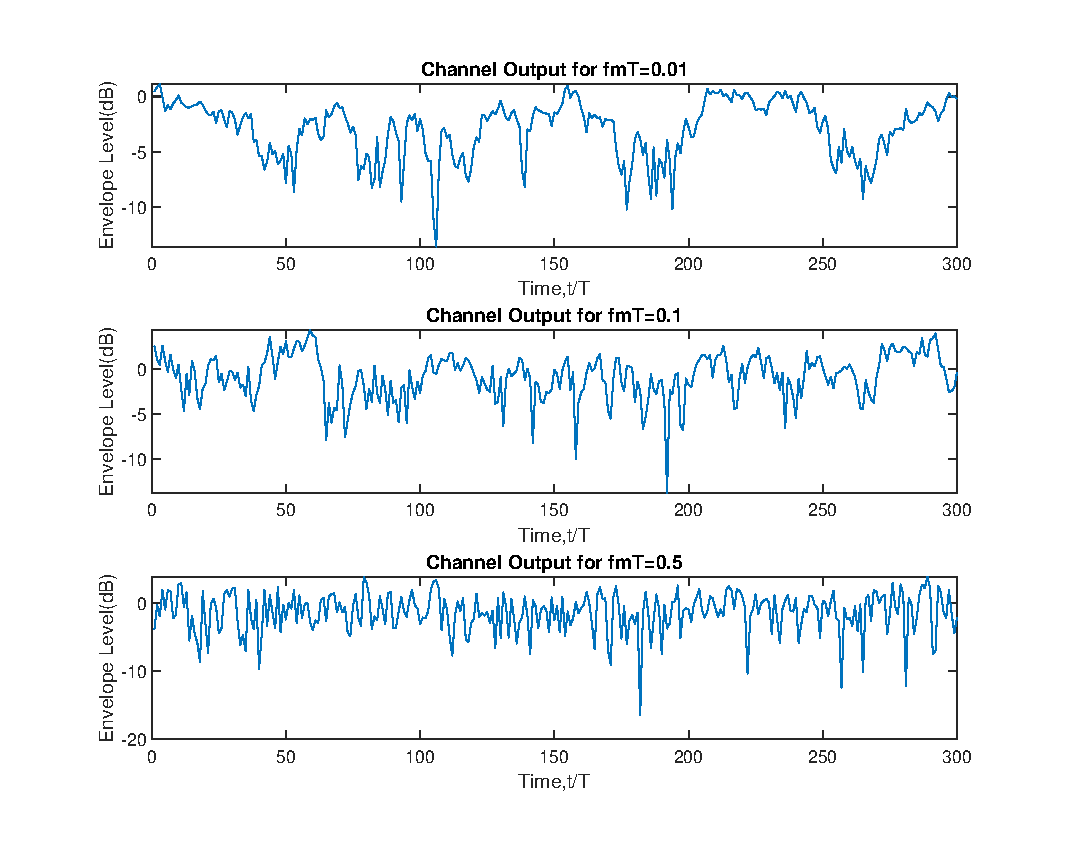
\includegraphics[scale = 0.7]{fg_envelop.eps}
\end{figure}
\begin{figure}[H]
    \centering
    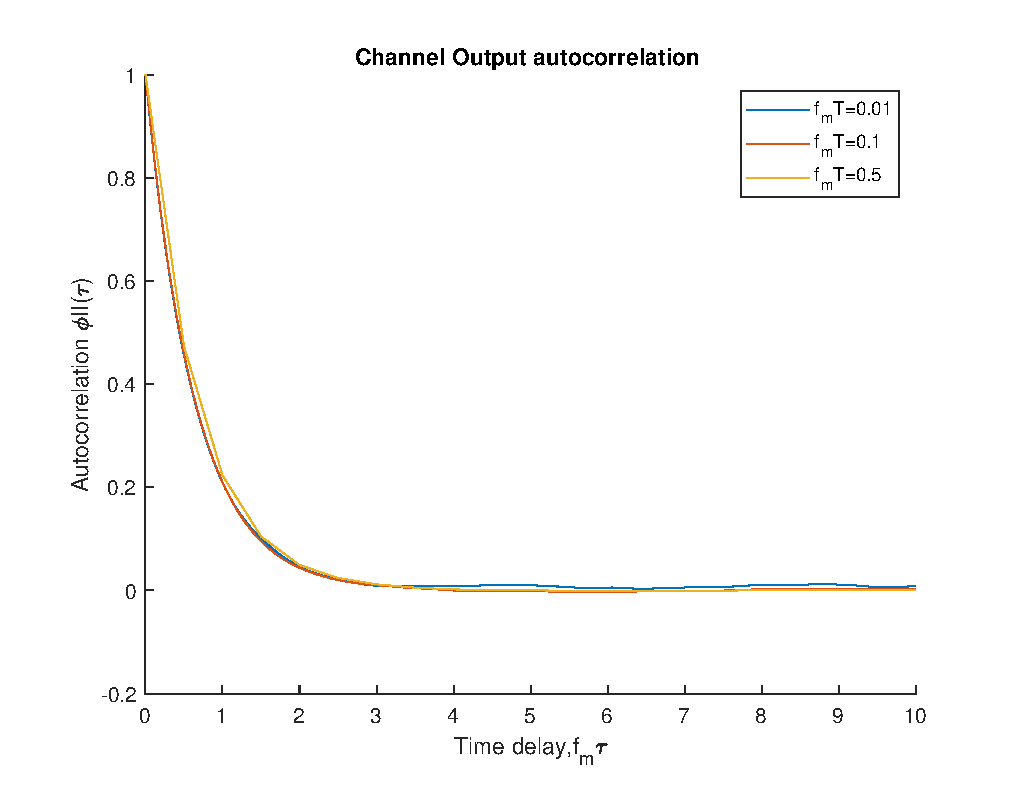
\includegraphics[scale = 0.7]{fg_auto.eps}
\end{figure}
    \item[{\bf 2. }]  \textbf{Radiation Pattern} \hfill \\
      \vspace{-10pt}
\begin{itemize}
    \item[(a)] No. Recall that one Erlang $\leftrightarrow$ one hour of call traffic during one gour of 
    operatiom. Therefore, the total traffic load cannot be greater than the number of available channel.
    \item[(b)] However, there are some results from (a) that do not satisfy the requirement above i.e $\rho >
    m$. The reason is that the actual traffic is determined by traffic load $\rho$ and blocking probability 
    $B(\rho, m)$, that is
    \begin{equation*}
        \text{actual traffic} = \hat{\rho} = (1 - B(\rho, m)) \rho
    \end{equation*}
\end{itemize}
    \item[{\bf 3. }]  \textbf{SIR for N = 16} \hfill \\
      
\begin{itemize}
    \item \textbf{Filtered Gaussian Noise method} \hfill \\
    In filtered gaussian noise method, we may notice that the fluctuation of the envelope 
    increases as $f_mT$ getting bigger. On the other hand, the auto correlation is not affected 
    by $f_mT$ a lot.
    \begin{itemize}
        \item Advantage: Different paths are uncorrelated.
        \item Disadvantage: This method is based on first-order filter. Therefore, the power 
        spectrum density of the generated siganl is much different from the ideal case (U shape).
        To have a more accurate result, we can use a higher order filter, which increases the complexity.
    \end{itemize}
    \item \textbf{Sum of Sinusoids method} \hfill \\
    In sum of sinusoids method, we may notice that the fluctuation of the envelope 
    increases as $f_mT$ getting bigger. Moreover, autocorrelation behaves more like the ideal 
    autocorrelation as $M$ increases. That is, for larger $M$, the undesired behavior occurs 
    later.
    \begin{itemize}
        \item Advanatges: generate isotropic scattering fading environment with low complexity 
        by using less oscillator.
        \item Disadvantage: There's no randomness in the generating process. Therefore, in order
        to use it for modeling the real case, some modification is needed. For example, different 
        simulation should start from different point to confront different fading.
    \end{itemize}
\end{itemize}
    \item[{\bf 4. }]  \textbf{SIR for N = 64} \hfill \\
      Similiar to that in (c), we may obtian the SIR for each signal under $N_r = 64$ received antenna.
The SIR of each signal is listed in the table below:
\begin{table}[H]
    \centering
    \begin{tabular}{c|c|c|c|c|c}
        & Signal 1 & Signal 2 & Signal 3 & Signal 4 & Signal 5 \\  
             \hline 
    SIR (dB) & 21.2980  & 16.7495  & 23.8789  & 21.1201  & 16.7325  
    \end{tabular}
\end{table}
Compared to that in problem 3, it can be observed that the SIR for 
each signal increases as the number of receiving antennas increases.
  \end{enumerate}
\end{document}
